\section{Scenarios as Message Sequence Charts}

Unlike labeled transition systems, that intrinsically model the behavior of a single agent (even if a composed one), scenarios explicitly illustrate interactions among multiple agents. The scenarios we use in this thesis are a syntactic subset of Message Sequence Charts (MSC)~\cite{ITU:1996} (see Fig.~\ref{image:train-scenario-all-agents} for example). To keep the models usable by end-users, however, we use only a small subset of their features. In its simplest form, a MSC is composed of vertical lines representing timelines associated with agents and horizontal arrows representing interactions among agents, also called \emph{events}. Following the modeling of agents of the previous section, events are synchronously sent and received by interacting agents (we also use the terms \emph{controlled} and \emph{monitored} events, respectively). As already stated in previous section, we assume that an event label uniquely determines the latter agents. 

We consider \emph{positive} scenarios, as examples of behaviors that the system should exhibit, in the next section and \emph{negative} scenarios, behaviors that the system must avoid, in the following one. Subsequent sections will then discuss ways of managing multiple positive and negative scenarios. 

\subsection{Positive scenarios}

The semantics of MSCs in this thesis is defined in terms of labeled transition systems, following~\cite{Uchitel:2003}. More precisely, MSCs define sets of event traces; we model the later with LTSs, as in previous section. Given a MSC, two kinds of traces can be considered: those from the local perspective of a single agent, and those from the global perspective of the composed system. Let us discuss the former first. As time in a MSC is represented top-down, the order in which events are sent and received along a particular timeline defines a total order. Therefore, from the perspective of a single agent, a MSC defines only one trace; precisely, one \emph{maximal} trace (that is, with all events to which the agent participates) and all its prefixes. For example, the traces seen by the \artifact{Controller} agent in the MSC of Fig.~\ref{image:train-scenario-all-agents} are precisely captured by the LTS of Fig.~\ref{image:local-traces-lts}. Given a MSC $M$ and an agent $Ag$, we denote such an LTS by $M_{\downarrow Ag}$.

\vspace{0.5cm}
\begin{figure}[H]\centering
\scalebox{0.45}{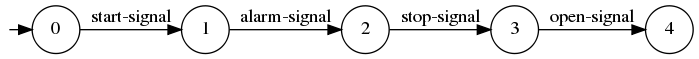
\includegraphics{src/2-framework/images/local-trace}}
\caption{LTS capturing the traces of the MSC of Fig.~\ref{image:train-scenario-all-agents} from the local point of view of the \artifact{Controller}.\label{image:local-traces-lts}}
\end{figure}

At first glance, a similar reasoning can be applied to the composed system. Indeed, one could consider that a MSC defines a \emph{maximal} trace in the composed system, with all events in a top-down ordering. In the example at hand, such a trace would be \artifact{<start-signal, start, alarm-pressed, \ldots, open>}. Making so amounts to consider that a MSC defines a total order among all events while it is commonly admitted that it defines only a partial order~\cite{ITU:1996, Uchitel:2003}. Consider for example the events \artifact{start-signal} and \artifact{alarm-pressed} at beginning of the MSC. These two events model unrelated phenomena between different agents, and can therefore hardly be considered timely ordered (e.g. maybe does the passenger push the alarm button when the \artifact{start-signal} is already sent but before \artifact{start} has been propagated? or even before \artifact{start-signal}?, and so on.). 

Even when considering partial ordering of all events, it is possible to capture all MSC traces respecting the total orders defined by the agent timelines. These traces are called \emph{linearizations} of the MSC. We do not formalize the structure of Message Sequence Charts and their linearizations here, and refer the reader to~\cite{Uchitel:2003} for such a mathematical characterization. Semantically, we note however that the set of system traces of a single MSC $M$ with $n$ interacting agents -- also called its \emph{language} -- can be constructively captured by the following LTS composition:

\begin{equation}
\label{equation:msc-composition}
\mathcal{L}(M) = \mathcal{L}(M_{\downarrow Ag_1} \parallel \ldots \parallel M_{\downarrow Ag_n})
\end{equation}

\noindent where, for recall, $M_{\downarrow Ag_i}$ denotes a LTS like the one of Fig.~\ref{image:local-traces-lts} for the timeline of the $i$-th agent. From an implementation point of view, the previous LTS composition gives a simple way of computing all linearizations of a MSC as a transition system directly. Such a LTS is illustrated in Fig.~\ref{image:msc-linearizations} for the case at hand, where six different linearizations exist due to the possible interleaving of the first four events. The reader familiar with the related literature may wonder here if some of these traces should not be considered as \emph{implied} scenarios. Strictly speaking, that is according to the definition of an implied scenario given in~\cite{Uchitel:2004}, they are not. We discuss implied scenarios in section \ref{section:background-discussion}.

\vspace{0.5cm}
\begin{figure}[H]\centering
\scalebox{0.31}{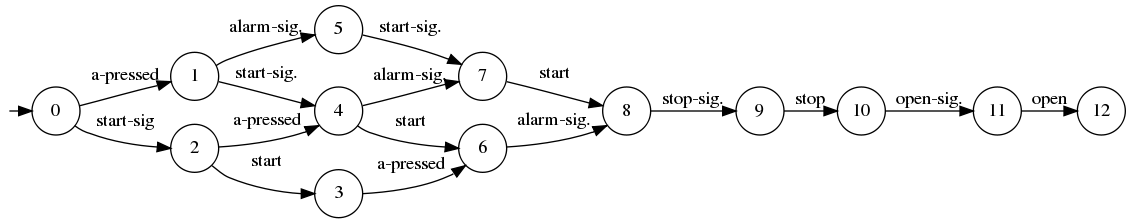
\includegraphics{src/2-framework/images/linearizations}}
\caption{LTS capturing all event linearizations of the MSC of Fig.~\ref{image:train-scenario-all-agents}. Here, \artifact{alarm-pressed} is abbreviated as \artifact{a-pressed} and \artifact{sig.} stands for \artifact{signal}. \label{image:msc-linearizations}}
\end{figure}

The semantics of a single MSC in terms of agent and system traces can now be explicitly related to the notion of the LTSs modeling the complete behavior of the agents and the system. That is, we can now explain the similitude between definitions \ref{equation:system-composition} and \ref{equation:msc-composition} through the notion of MSC consistent with a system. 

Consider a system $S$ composed of $n$ agents whose behavior is modeled by the LTSs $Ag_1$ to $Ag_n$. Let $M$ denote a MSC illustrating interactions between them. We say that $M$ is \emph{consistent} with $S$ -- or, more accurately, that $M$ and $S$ \emph{are} consistent -- if the following conditions hold:

\begin{itemize}
\item $M$ and $S$ are \emph{architecturally} consistent,
\item $\mathcal{L}(M_{\downarrow Ag_i}) \subseteq \mathcal{L}(Ag_i)$ for each agent $Ag_i$, and
\item $\mathcal{L}(M_{\downarrow Ag_1} \parallel \ldots \parallel M_{\downarrow Ag_n}) \subseteq \mathcal{L}(Ag_1 \parallel \ldots \parallel Ag_n)$
\end{itemize}

The first condition is not formalized but simply requires the MSC and the system to agree on the set of agents (a MSC may actually illustrate interactions among a proper subset of system agents) and their respective interfaces (labels along a timeline are a subset of the alphabet of the corresponding agent). The second condition states that the traces defined by a timeline in the MSC must be traces accepted in the LTS modeling the behavior of the corresponding agent. The third condition states that all linearizations of the MSC must be accepted traces of the LTS modeling the behavior of the composed system. Note that, under architectural consistency, the second condition implies the third one~\cite{Uchitel:2003}. Last, but not least, stated conditions restrict consistent MSCs to those starting in the system initial state.

\subsection{Negative scenarios}

While positive MSCs model examples of behavior that the system is expected to exhibit, it is often convenient to be able to model the counterpart, that is examples of behavior that the system is expected (even required) \emph{not} to exhibit. Such proscribed behaviors are illustrated with negative MSCs~\cite{Uchitel:2004}. A negative MSC is simply a scenario whose last event is proscribed, as depicted by a crossed arrow below a dashed line. An example is given in Fig.~\ref{image:train-negative-scenario}, where the \artifact{Controller} may not open doors immediately after having started the train.

\vspace{0.4cm}
\begin{figure}\centering
\scalebox{0.75}{
  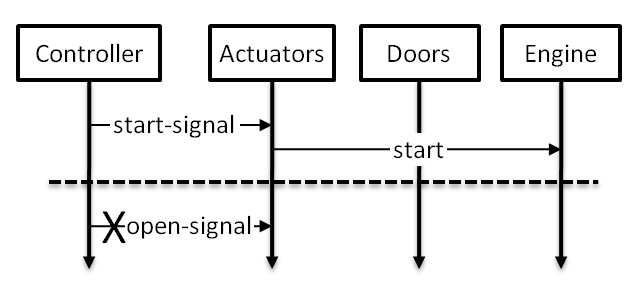
\includegraphics[trim=2mm 2mm 2mm 2mm, clip]{src/2-framework/images/train-negative-scenario}
}
\caption{A negative scenario illustrating that the controller may not open doors after having started.\label{image:train-negative-scenario}}
\end{figure}

More precisely, a negative MSC is a pair $(P,e)$ where $P$ is a positive MSC and $e$ is a single event (given our simplifying assumption, the latter event can simply be denoted by its label $l = label(e)$). The positive scenario $P$ is called the $precondition$ and $e$ the \emph{proscribed event}. The intuitive semantics is that, once the precondition has occurred from the system initial state, $e$ may not be the (very) \emph{next} event in the system. We make this semantics fully precise now. A negative MSC $N = (P,e)$ defines a set of traces as follows:

\begin{equation*}
\mathcal{L}(N) = \{~w.l \mid w \in \mathcal{L}(P) \wedge l = label(e)~\}
\end{equation*}

That is, traces of a negative MSC are traces of the precondition (given by definition~\ref{equation:msc-composition}) concatenated with the label of the proscribed event. Note that such a definition implies that the precondition must occur completely for the proscribed event to be taken into account. In other words, partial orderings between the proscribed event and those in the precondition are not considered. This is the intended meaning of the dashed line separating them~\cite{Uchitel:2004}. In contrast, note that all linearizations of the precondition are taken into account (even if the MSC of Fig.~\ref{image:train-negative-scenario} presents only one). 

Similarly to positive MSCs, we state conditions for a negative MSC $N = (P,e)$ and a system $S = (Ag_1 \parallel \ldots \parallel Ag_n)$ to be consistent, as follows:

\begin{itemize}
\item $N$ and $S$ are \emph{architecturally} consistent,
\item $P$ and $S$ are consistent, and
\item $\mathcal{L}(N) \not\subseteq \mathcal{L}(Ag_1 \parallel \ldots \parallel Ag_n)$
\end{itemize}

The first condition is similar to what has been said previously for positive MSCs. The second enforces the precondition to be a consistent (positive) MSC. The last one states that the system may not exhibit any trace captured by the negative MSC.

\subsection{Scenario collection}

Systems are generally illustrated with multiple positive and negative scenarios. The most straightforward way of doing so is through scenario collections $Sc = (S^+,S^-)$ where $S^+$ and $S^-$ are (possibly empty) sets of positive MSCs and negative MSCs, respectively. It is straightforward, yet useful, to extend the notions of language and consistency of scenarios to collections of them. 

The positive and negative languages defined by a scenario collection $Sc = (S^+,S^-)$ are simply defined via the union on languages:

\begin{center}
$\mathcal{L}^+(Sc) = \bigcup_{P \in S^+} \mathcal{L}(P)$ \\
$\mathcal{L}^-(Sc) = \bigcup_{N \in S^-} \mathcal{L}(N)$
\end{center}

Also, a scenario collection and a system are said to be consistent if and only if each positive and each negative MSC of the collection is itself consistent with the system. We extend this to the consistence of the collection of scenarios itself as follows: two sets of positive and negative scenarios, $S^+$ and $S^-$, are consistent with each other if there exists a system which is consistent with them taken as a collection $Sc = (S^+,S^-)$. A necessary condition for a scenario collection to be consistent (but not sufficient, because architectural consistency is not taken into account here) is the disjointness of positive and negative traces:

\begin{center}
$Sc = (S^+,S^-)$ is consistent only if $\mathcal{L}^+(Sc) \cap \mathcal{L}^-(Sc) = \emptyset$
\end{center}

Note that, by definition, a collection cannot be consistent with a system unless all scenarios start in its initial system state. Also, a (finite) scenario collection is hardly complete in practice, in the sense that it cannot describe all system behaviors (most system accept an infinite number of traces, through loops). Last, multiple scenarios starting in the same initial state imply a lot of redundancy in system descriptions, which renders refactoring difficult in practice. High-level Message Sequence Charts (hMSCs), introduced in the next section, provide a mean to tackle these three problems.

\subsection[Flowcharting scenarios in high-level MSCs]{Flowcharting scenarios in high-level Message Sequence Charts}

High Level Message Sequence Charts are directed graphs where each node refers to a MSC (named \emph{basic} MSC here, bMSC for short) or a finer grained hMSC. Outgoing edges of a node capture its possible continuations, allowing the user to introduce sequences, alternatives and loops, to reuse small MSC fragments, and so on. An hMSC also has an initial starting point that indicate the initial system state. An example of hMSC is given in Fig.~\ref{image:train-hmsc}.

\vspace{0.4cm}
\begin{figure}[H]\centering
\scalebox{0.65}{
  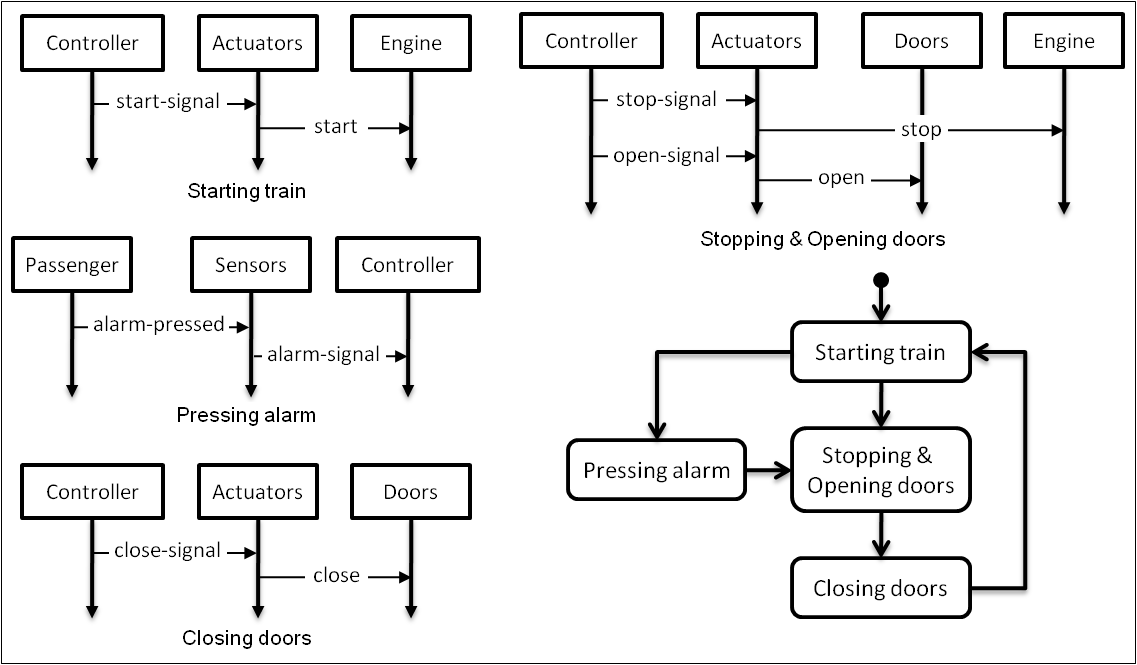
\includegraphics[trim=2mm 2mm 2mm 2mm, clip]{src/2-framework/images/train-hmsc}
}
\caption{A high-level Message Sequence Chart for the train system.\label{image:train-hmsc}}
\end{figure}

